\section{Assessment}\label{sec:assessment}
In order to evaluate the strength of our different player strategies, we first ran them in a local server, a feature implemented in \cite{poke_env}, that simulates a player vs player battle. It did not work out of the box due to some incompatibilities between the Node JS version and the Python one, so, in order to solve this problem and to improve reproducibility, we wrote a Docker \cite{merkel2014docker} file that is available in the root of the GitHub repository. The poke-env library \cite{poke_env} implements a "baseline" player that has an Elo rank of 1100-1200 points on the remote server \cite{showdown_competition}. So, our aim was to develop at least two players, a rule-based (\autoref{subsec:rule_based_player}) and a minimax (\autoref{subsec:minimax_player}), that could defeat it. Then, we made them battle against each other a thousand of times to assess their strength. At this point, it faced out that the mini-max player made too many \poke switches, so we developed a new strategy in which we exclude them from the mini-max tree computation. In \autoref{fig:minimax_without_switches} we can see the differences with respect to the approach described in \autoref{subsec:minimax_player}. In this way, the player chooses whether or not switch a \poke at the beginning of each turn, only based on the matchup score, just like the rule-based player does.

So, going back to performances between each player, we can declare, by looking at \autoref{tab:win_percentage_players}, the rule-based and minimax players to be the best ones as expected.
\begin{table}[!htbp]
    \footnotesize
    \centering
    \begin{tabular}{c|c|c|c|c}
        \hline \hline
         \textbf{Player} & \textbf{MBP} & \textbf{BD} & \textbf{RB} & \textbf{MM} \\ \hline \hline
         \textbf{MBP} & / & 0.104 & 0.084 & 0.114 \\ \hline
         \textbf{BD} & 0.896 & / & 0.398 & 0.452 \\ \hline
         \textbf{RB} & 0.916 & 0.602 & / & 0.571 \\ \hline
         \textbf{MM} & 0.886 & 0.548 & 0.429 & / \\ \hline \hline
    \end{tabular}
    \caption{Percentage of win for every player against each other}
    \label{tab:win_percentage_players}
\end{table}

We have also noticed some more things: first of all using the matchup function for choosing the best switch increased the performance of about $5\%$ (with a proper switch strategy of course) against the baseline player from \cite{poke_env}, while using the gimmick strategy had the major effect with a $8$-$9\%$ increase in performance.

As a final test, we run our two best players for $100$ matches on the remote server \cite{remote_server} against human players on generation $8$ random battles. We can look at their ELO progression in \autoref{fig:elo_players}.
\begin{figure}[!htbp]
    \centering
    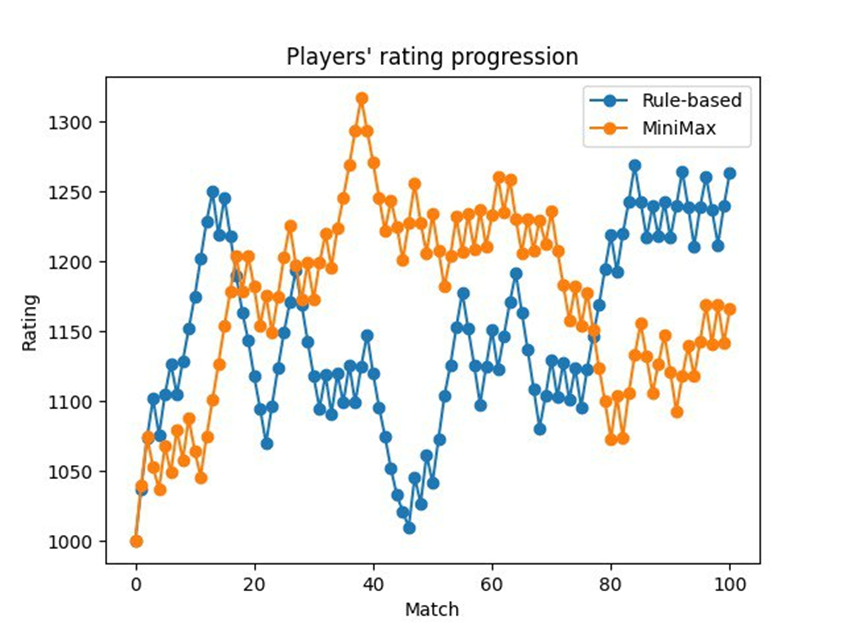
\includegraphics[width=0.8\linewidth]{images/elo_players.png}
    \caption{ELO progression of RB and MM players against human players}
    \label{fig:elo_players}
\end{figure}
It turns out that the two players float around the $1200$ ELO points, making them somewhat at the level of an average skilled human player.
